\section{Important Concepts}
\label{sec:concepts}

To identify the names of a variable, our approach first is to examine
its own {\bf attributes and behaviors} via field accesses and method calls
in the given source code. Then, we examine the {\bf relations} of the
variables within the context of the method/function to learn the
concordance among the variables' names via the usages of the variables
in the code. Finally, we examine the {\bf relations among the types}
of variables. Let us explain those concepts used in {\tool}.

\begin{definition}{\bf [Attributes and Behaviors]}
  The fields and methods of the object represented by a variable are
  referred to as the attributes and behaviors, respectively. The names
  for those fields and methods of a variable are intact after code
  minification.
%The properties of a variable are not minified: its accessible fields
%representing the attributes and its accessible methods representing
%the behaviors performed by the corresponding object.
\end{definition}

%From Observation 1, we can rely on the names of the fields and those
%of the methods accessed from a variable as an important pivot in
%order to recover the name of the variable.  A model can encounter the
%same names for the fields and methods, it can learn to derive the
%name of the variable under study because the names of the variable
%and those of the methods and fields in the original code are in
%harmony with one another. For example,

In Figure~\ref{example_sim}, at lines 7--9, we explore the
field accesses and method calls of the variable \code{r} in
\code{r.cloneRange()}, \code{r.startOffset}, and \code{r.endOffset}.

We denote an instance of field access and method call as a triple $(v,
p, t)$, where $v$ is the variable, $p$ is the name of the field or
method, and $t$ is either \code{fieldAccess} or \code{methodCall}.
The examples include $(r, cloneRange, methodCall)$ and $(r,
startOffset, fieldAccess)$.


%Tien

\begin{definition}{\bf [Argument Relation]}
  A variable $v$ is said to have an argument relation with a method
  $m$ if it is used as an argument of a call to that method as in
  $o.m(...,v,...)$.
\end{definition}

\begin{definition}{\bf [Assignment Relation]}
  A variable $v$ is said to have an assignment relation with a method
  $m$ or a field $f$ if it is used as a left-hand side in an
  assignment from a method call or a field access as in $v =
  o.m(...)$, or $v = o.f$.
\end{definition}


%
%We focus on the roles of a variable used {\em as an argument in a method call}
% or {\em receiving the value returned by a method call or field access}.
%
%If we have $o.m(...,v,...)$, $v = o.m(...)$, or $v = o.f$,
%where $m$ is a method call and $f$ is a field access,
%then there exist
%the role relations between $v$ and $m$, and between $v$ and $f$.

The idea is that the name of the minified variable $v$ in the original
code is often in accordance with the names of the method or the field
in such an assignment or an argument. For example, \code{range} and
\code{getRangeAt} are in accordance with each other in \code{range =
  selection.getRangeAt(0)}; or \code{selectNodeContents} and
\code{root} are in accordance with each other in
\code{preSelectionRange.selectNodeContents(root)}.  We will use the
triple notations $(v, p, argument)$, $(v, p, assignment)$, and
$(v, f, assignment)$ to denote those three cases, where $v$ is a
variable, $p$ is a method name, and $f$ is a field name.

%The rationale is that the names of $m$ and its argument are often in
%conformance with each other, \eg
%\texttt{getData(contentType)}. Similar rationale is applied to the
%above assignments to $v$.

%A variable could be received a value of a field/method, or could be a
%input of an method invocation. For instance, in
%figure \ref{example_sim}, variable \texttt{r} receives the result of
%an assignment to the boolean expression $t.clipboardData ||
%a.clipboardData || e.dataTransfer$. In case of variable \texttt{f}, it
%is an argument of function \texttt{getData()} and the value
%of \texttt{getData()} is influenced by \texttt{f}.

%A role relation between a variable \texttt{v} and a field/method
%\texttt{p} is denoted by a triple $(v, p, t)$, where
%\texttt{t} is the type of role relation. A role relation could
%be either \texttt{argument} or \texttt{assignment}.

%We expect this role relation to contribute significantly to the name
%recovery process.
%%
%%This type of relation also contributes remarkably in reducing the name
%%searching space when recovering a variable.
%For example, a variable \texttt{x} in a minified code is assigned with
%the value of a field access to \texttt{httpBody} and is used as an
%argument in a call to \texttt{setBodyHttp()}. In our dataset, there
%are only 19 variable names that are assigned with the value
%of \texttt{httpBody}, while the number
%%of variable names is used for method call
%with regard to \texttt{setBodyHttp()} is 11.
%%The figure for names having both two relations is only 5.
%Then, there are only 5 candidate names that satisfy both conditions.
%Thus, our algorithm could reduce the number of candidates from +200K
%to only 5.
%%Therefore, the number of variable names could be recovered
%%for \texttt{x} reduced down to 5 in comparison with about 200k
%%variable names of our corpus.



%In our scope, we consider 2 common data dependency between
%variable \texttt{x} with fields, methods, which is shown in
%table \ref{table:DataDep} as below.

%\begin{table}[h!]
%\begin{tabular}{|c|c|c|c| }
% \hline Sample & Variable & Methods/Fields & Dependency Type \\
% [0.5ex] \hline x = Http.httpBody & x & httpBody &
% Assignment \\ \hline t.setBodyHttp(x) & x & setBodyHttp() &
% Argument \\ \hline
%\end{tabular}
%\caption{Data dependency}
%\label{table:DataDep}
%\end{table}


\begin{definition}{\bf [Relation Graph]}~\cite{icse19}
A relation graph (RG) is a directed graph
%in the shape of a star to represent the single-variable usage context
%of $v$ with regard to its property and role relations with 
%the fields and methods in its usage.
%
in which each node of the RG represents a variable. The connected
nodes represent the methods/fields in method calls or field accesses,
respectively, and are labeled with their names. Edges represent
relations among nodes and are labeled with relation types.
\end{definition}

%Figure~\ref{SG_sample_ano} shows the relation graph of the variable
%\texttt{r}, which includes a set of property relations:
%$( \texttt{r}, \texttt{types}, \texttt{fieldAccess})$, $( \texttt{r},
%\texttt{getData}, \texttt{fieldAccess})$, $( \texttt{r},
%\texttt{getData()}, \texttt{methodCall})$,
%
%and a set of role relations: $( \texttt{r}, \texttt{clipboardData},
%\texttt{assignment})$, $( \texttt{r}, \texttt{dataTransfer},
%\texttt{assignment})$ in our example.

\begin{figure}[t]
	\begin{center}
	  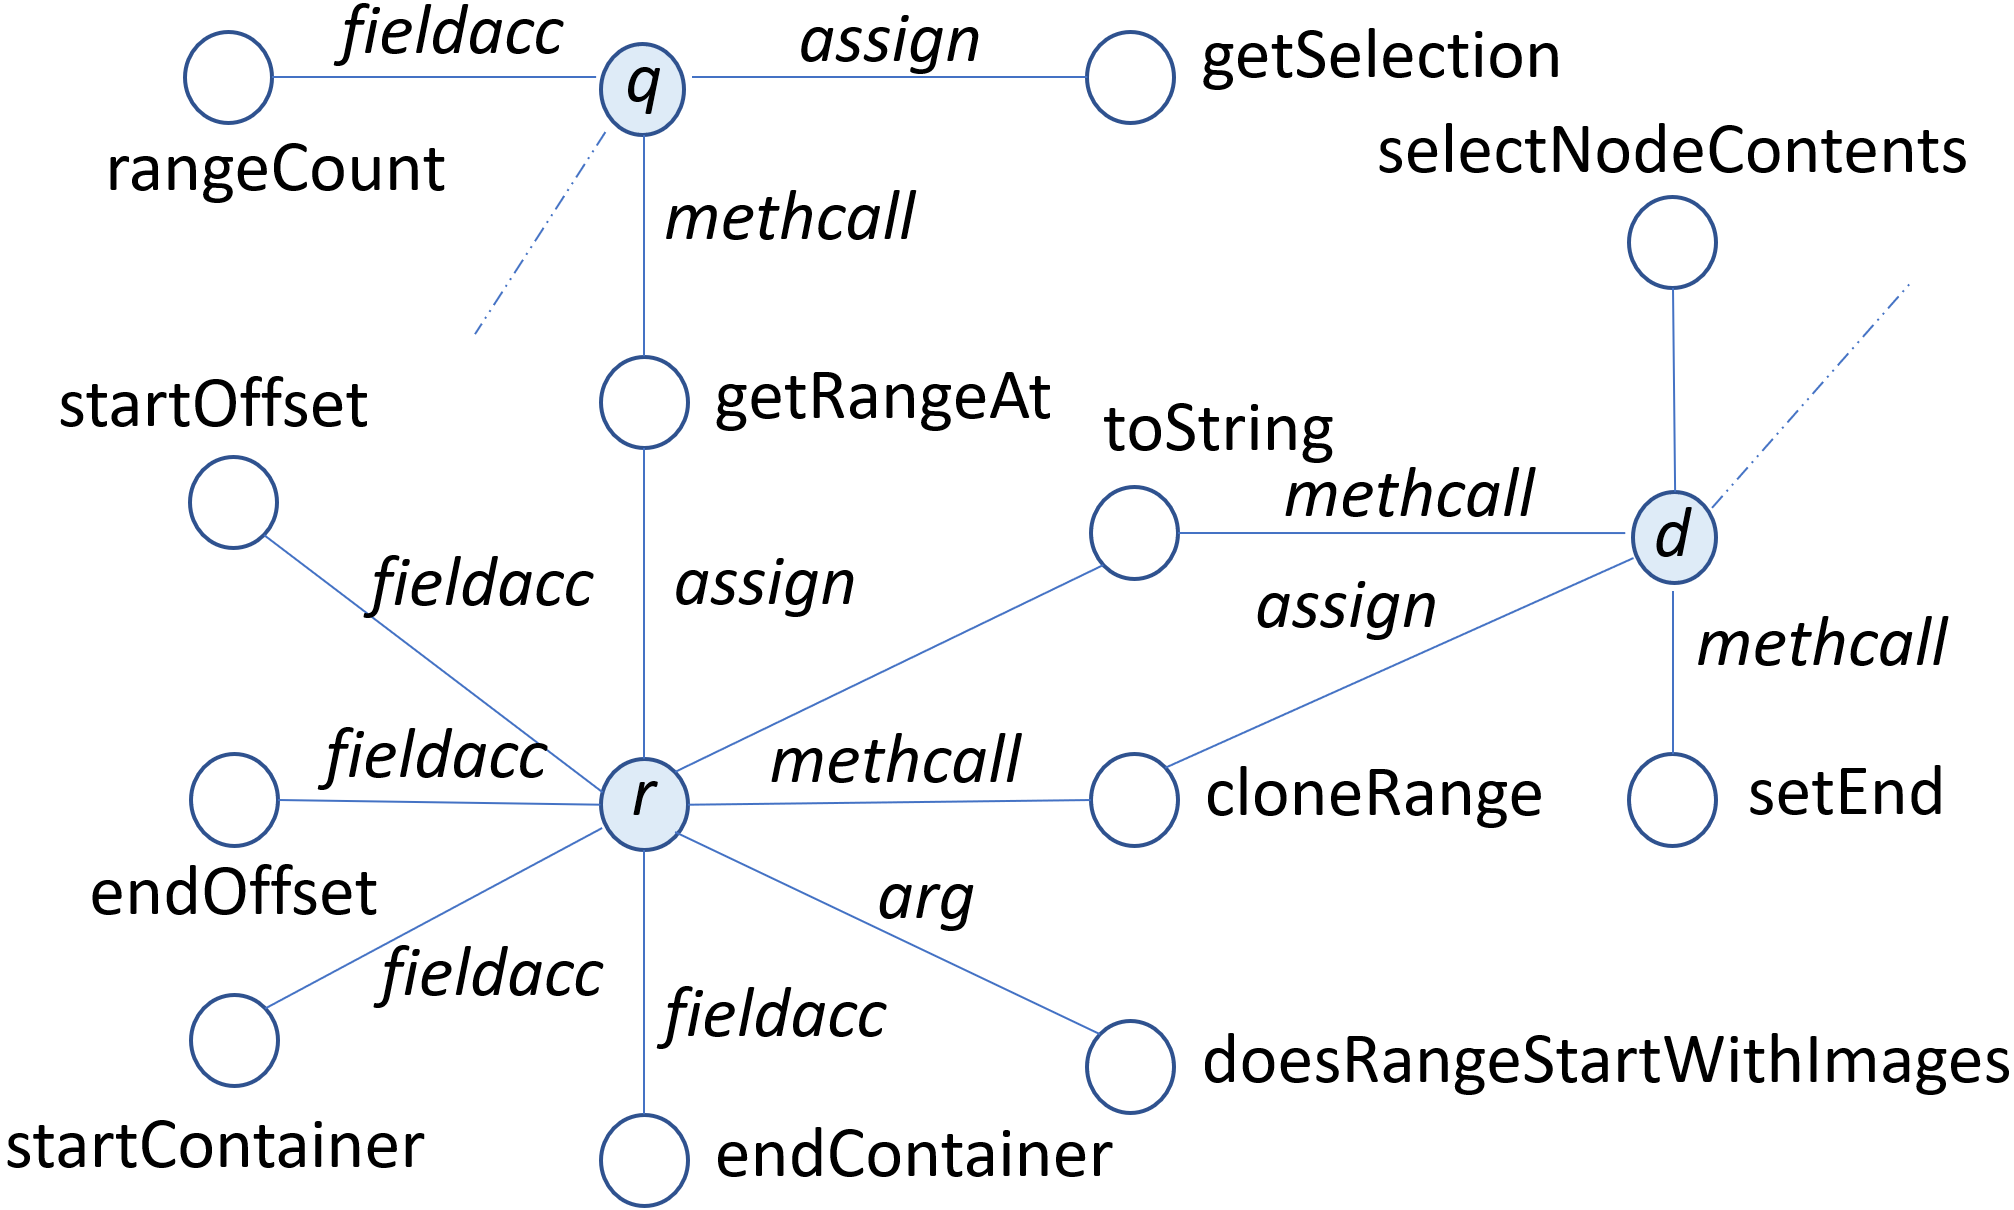
\includegraphics[width=0.9\columnwidth]{figures/relation-graph}
          \vspace{-6pt}
		\caption{Relation Graph for Figure~\ref{example_sim}}
		\label{rel-graph}
	\end{center}
\end{figure}

Figure~\ref{rel-graph} shows the relation graph for the variables in
the code in Figure~\ref{example_sim}. For example, there are an
$assign$ edge from the variable \code{r} to the node
\code{getRangeAt}, and a $methodcall$ edge from \code{q} to
\code{getRangeAt} because we have \code{r = q.getRangeAt(0)} at line
6.




\begin{figure}[t]
  \small
  \begin{eqnarray*}
    \theta \in Type (\Theta) &::=& \gamma | \, \alpha [\theta, ..., \theta] \, | \, u \, | \, \mathbf{None} \, | \, \mathbf{type}\\
  \gamma \in \, Elementary \, Type (\Gamma) &::=& \mathbf{int} \, | \, \mathbf{float} \, | \, \mathbf{str} \, | \, \mathbf{bool} \, | \, \mathbf{bytes}\\
  \alpha \in Generic \, Type (A) &::=& \mathbf{List} \, | \, \mathbf{Tuple} \, | \, \mathbf{Dict} \, | \, \mathbf{Set} \, |\\
  & & \, \mathbf{Callable} \, | \, \mathbf{Generator} \, | \, \mathbf{Union}\\
  b \in \, Builtin \, Type (B) &::=& \gamma \, | \, \alpha[\theta]\\
  u \in \, User \, Defined \, Type (U) &::=& all \, classes \, and \, named \, tuples\\
  o \in \, Overloading \, User \, Def \, Type (O) &::=& all \, classes \, with \, operator \\
  & & overloading \, in \, code
  \end{eqnarray*}
  \vspace{-18pt}
\caption{Types in Python}
\label{python-types}
\end{figure}

In this work, we focus on Python source
code. Figure~\ref{python-types} shows Python's type
system~\cite{type-graph-icse22}. To represent the dependencies among
the types, we adopt Type Dependency Graph
(TDG)~\cite{type-graph-icse22}, which aims to capture the type
inference rules for variables/expressions.

\begin{definition}{\bf Type Dependency Graph]}~\cite{type-graph-icse22}
    \label{tdg-def}
A Type Dependency Graph is a graph $G$ = $(N,E)$ in which $N$ is the
set of nodes representing all the variables and expresions, and $E$ is
the set of edges from $n_i$ $\rightarrow$ $n_j$ indicating that the type of $n_j$
can be derived from the type of $n_i$ by the type inference rules in
the type system.
\end{definition}

In Figure~\ref{example_sim}, let us consider line 4: \code{q =
  b.getSelection()}. The TDG will contain a node for the expression
\code{b.getSelection()} connecting to a node for the variable \code{q}
because its type can be derived from the return type of the method
call \code{getSelection}. We also have a node for the variable
\code{b} connecting to a node the method \code{getSelection}
because the type of \code{getSelection} can be derived from
that of the variable \code{b}.

\fbox{\code{b.getSelection}} $\rightarrow$ \fbox{\code{q}}

\fbox{\code{getSelection}} $\rightarrow$ \fbox{\code{b}}

%For example, from line 10 of Figure~\ref{example_org}, \code{start} =
%\code{preSelectionRange.} \code{toString().} \code{length}, our model
%can build the dependency between the type of \code{start} from the
%type of \code{length} in the \code{String} class (which is
%\code{int}). As another example, there is a type dependency between
%the return type of \code{getIndexRelativeToAdjacentEmptyBlocks} and
%the type of the variable \code{emptyBlocksIndex} at line 23:
%\code{emptyBlocksIndex} \code{=}
%\code{this.get\-Index\-Relative\-To\-Adjacent\-Empty\-Blocks(...)}.
%another dependency between the type of \code{emptyBlocksIndex} and the
%type of \code{selectState.emptyBlocksIndex} at line 25.
Connecting all the dependencies among the types of variables and
expressions, we have the type dependency graph for a
function/method. Note that both the Type Dependency Graph and the
Relation Graph can be built for either the original or minified code.

%We leverage the graph building algorithm from HiTyper to parse the
%code and transform every variable occurrence and expression into nodes
%and maintains type dependencies between them. We also extend the
%notion and the algorithm to build the type dependency graph (TDG) for
%the JavaScript code. Details on TDG is in~\cite{type-graph-icse22}.


\begin{figure}[t]
	\begin{center}
	  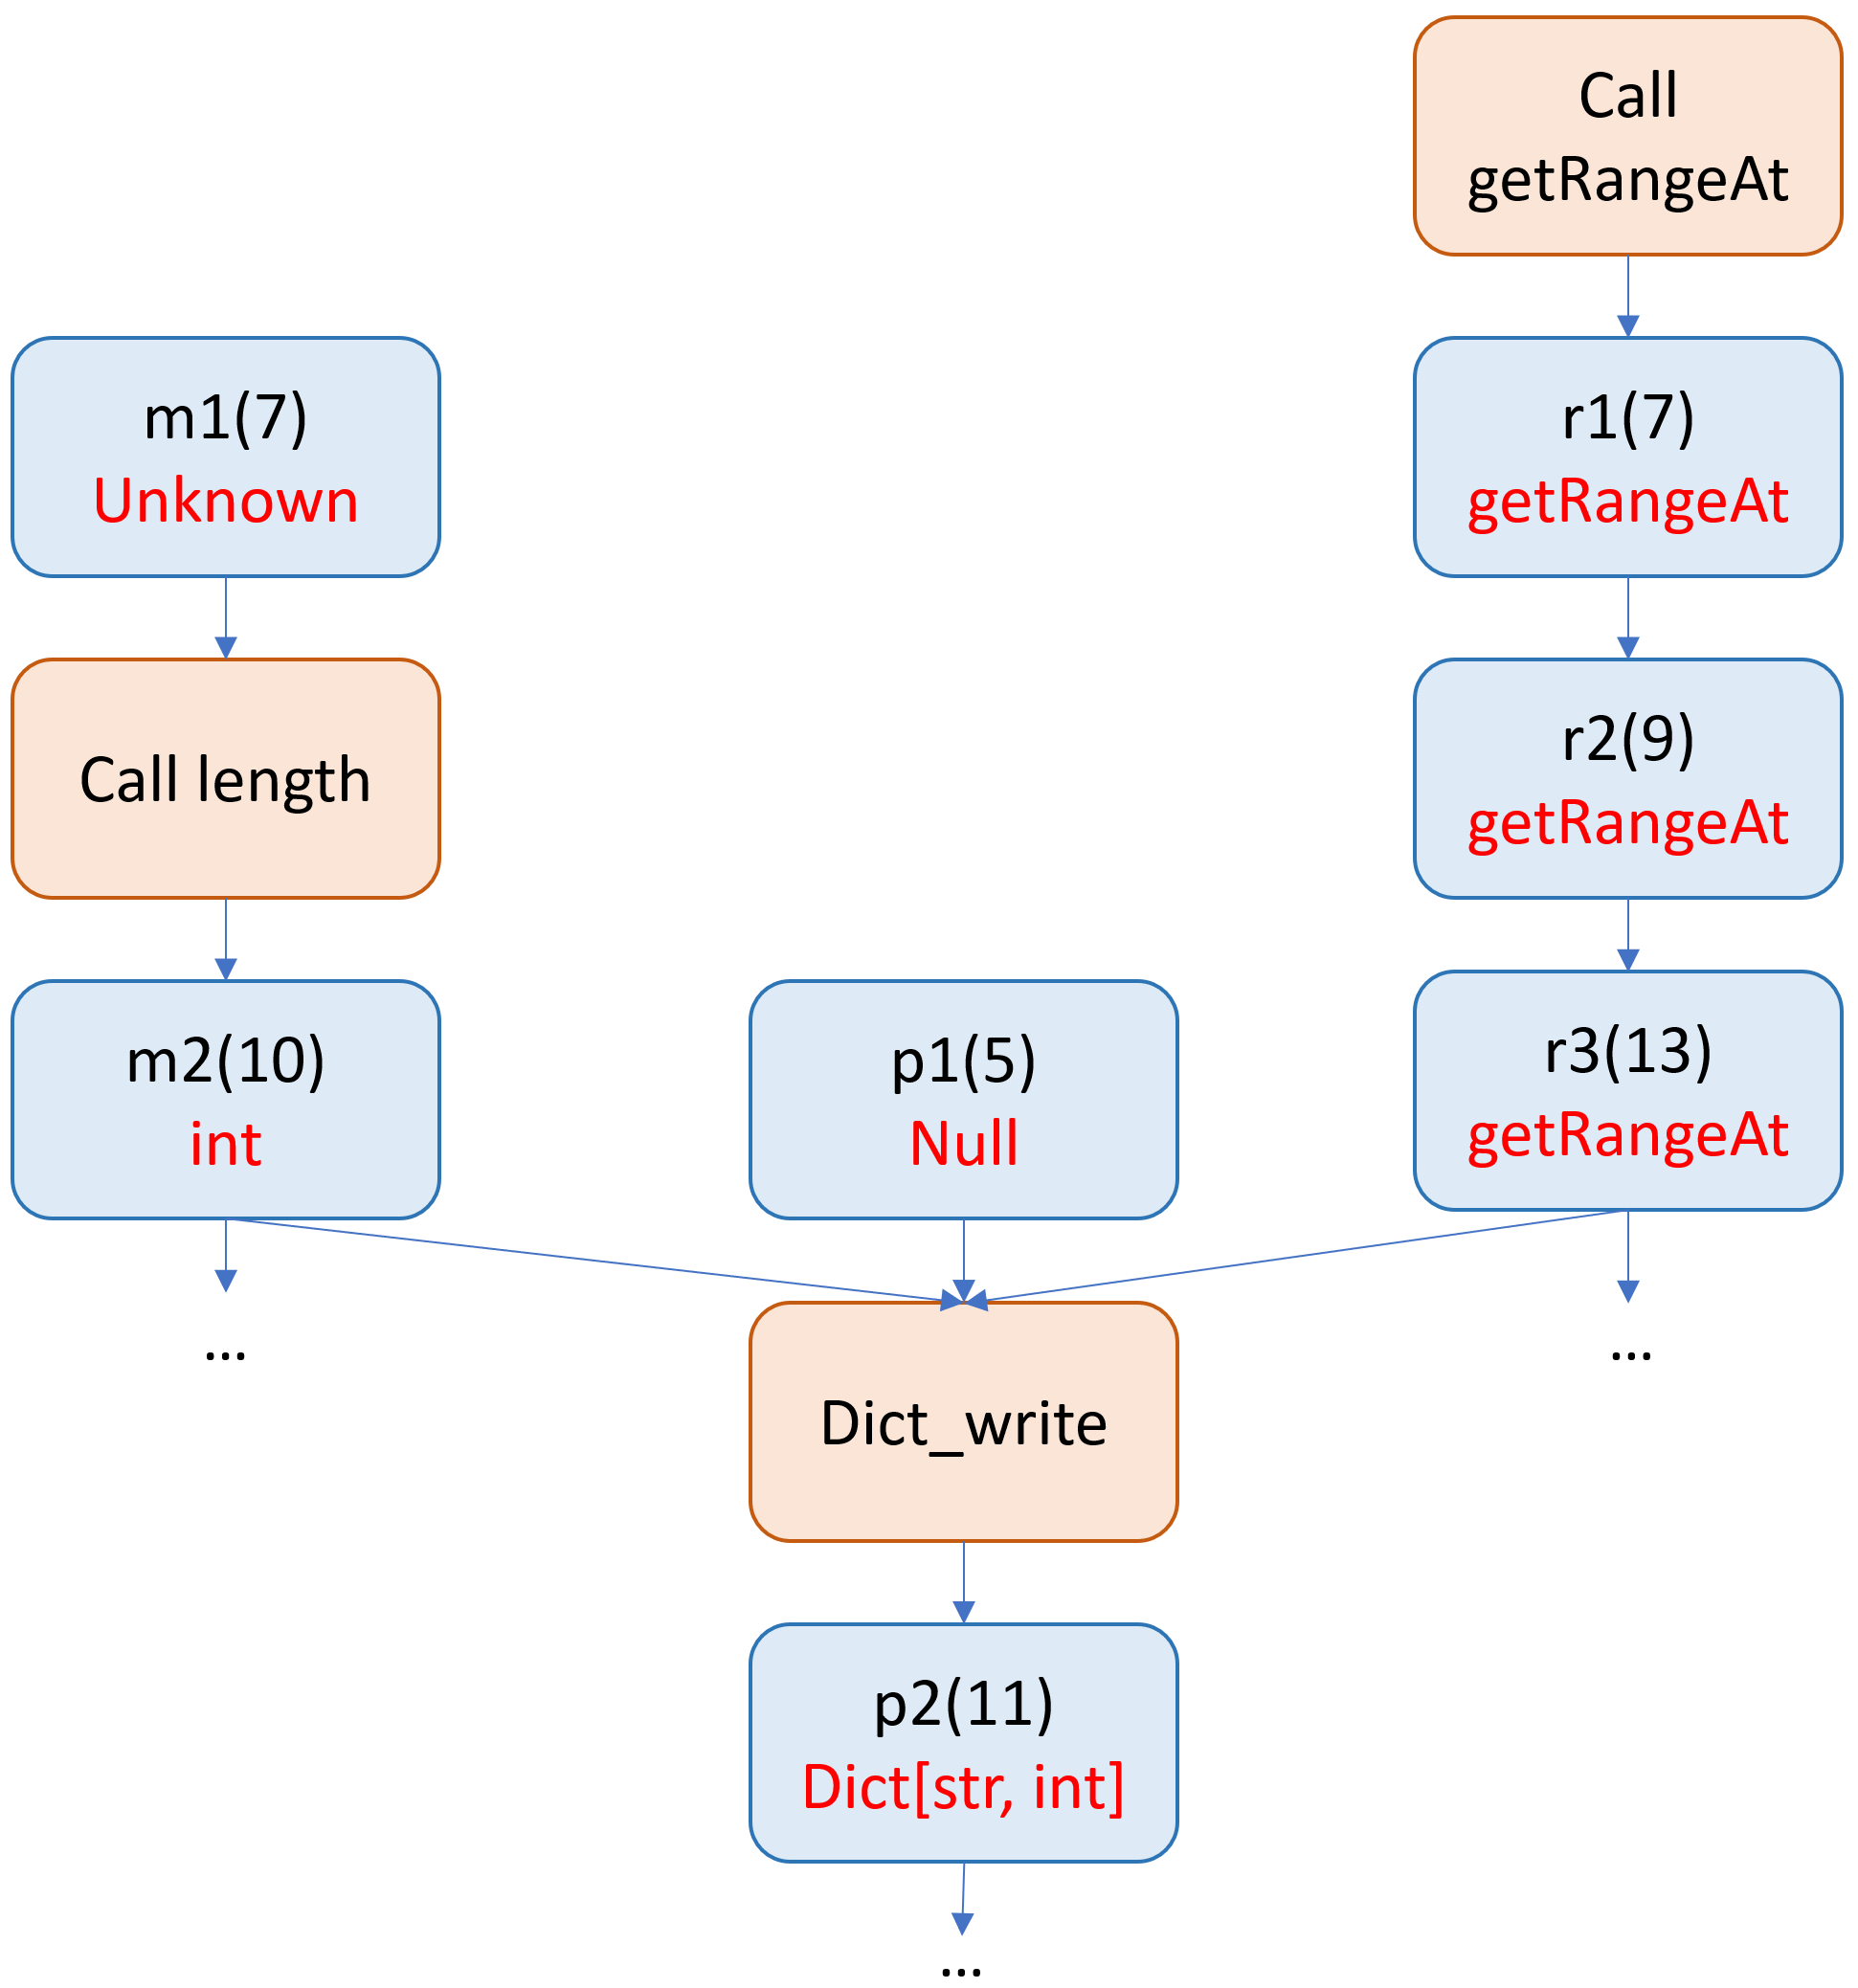
\includegraphics[width=1.8in]{figures/type-dep-graph}
          \vspace{-8pt}
		\caption{Type Dependency Graph for Figure~\ref{example_sim}}
		\label{tdg}
	\end{center}
\end{figure}

Figure~\ref{tdg} displays the TDG for the running example. While the
variable $m$ at line 7 (Figure~\ref{example_sim}) has unknown type,
its type at line 10 can be derived by the function call
\code{length}. At line 11 (Figure~\ref{example_sim}), the type of the
variable \code{p} is derived from the type of the left-hand-side of
line 11 (\code{Dict}). Thus, we have an edge from \code{Dict\_write}
to \code{p}.
